% Compile with XeLaTeX twice from this directory.
\documentclass[10pt,a4paper]{article}
\usepackage{fontspec,unicode-math}
\setmainfont{TeX Gyre Termes}
\setsansfont{TeX Gyre Heros}[Scale=MatchLowercase]
\setmonofont{Latin Modern Mono}[Scale=0.82]
\setmathfont{STIX Two Math}
\usepackage[margin=22mm,headheight=14pt]{geometry}
\usepackage{microtype,booktabs,graphicx,amsmath,xcolor,hyperref,fancyhdr,enumitem}
\usepackage{xurl}
\usepackage{tikz}
\usepackage{pgfplots}
\pgfplotsset{compat=1.18}
\usetikzlibrary{arrows.meta,positioning}
\definecolor{accent}{HTML}{175A63}
\definecolor{cachelight}{HTML}{9BBBC0}
\definecolor{outputgold}{HTML}{BA8744}
\hypersetup{colorlinks=true,urlcolor=accent,linkcolor=accent,citecolor=accent,
  pdftitle={HCCA for Token-Efficient Repository Repair},pdfauthor={HCCA Project}}
\setlength{\parskip}{3pt}
\setlength{\parindent}{1em}
\setlist{nosep,leftmargin=*}
\pagestyle{fancy}
\fancyhf{}
\fancyhead[L]{\small\sffamily HCCA for Token-Efficient Repository Repair}
\fancyhead[R]{\small\sffamily Technical report}
\fancyfoot[C]{\small\thepage}
\renewcommand{\headrulewidth}{0.3pt}
% Derived from the versioned November 12 and November 13 public summaries.
\newcommand{\HRequests}{1,301}
\newcommand{\HInput}{36,810,516}
\newcommand{\HCached}{35,849,984}
\newcommand{\HMiss}{960,532}
\newcommand{\HOutput}{654,304}
\newcommand{\HReasoning}{408,903}
\newcommand{\HOtherOutput}{245,401}
\newcommand{\HCachePct}{97.3906}
\newcommand{\HCost}{0.644212152}
\newcommand{\HCostPerResolved}{0.017895}
\newcommand{\LRequests}{1,061}
\newcommand{\LInput}{29,253,597}
\newcommand{\LCached}{28,189,696}
\newcommand{\LMiss}{1,063,901}
\newcommand{\LOutput}{516,149}
\newcommand{\LReasoning}{365,085}
\newcommand{\LOtherOutput}{151,064}
\newcommand{\LCachePct}{96.3632}
\newcommand{\LCost}{0.553843638}
\newcommand{\LCostPerResolved}{0.016290}
\newcommand{\BRequests}{2,014}
\newcommand{\BInput}{106,265,446}
\newcommand{\BCached}{104,137,856}
\newcommand{\BMiss}{2,127,590}
\newcommand{\BOutput}{4,050,837}
\newcommand{\BReasoning}{3,690,753}
\newcommand{\BOtherOutput}{360,084}
\newcommand{\BCachePct}{97.9979}
\newcommand{\BCost}{3.062054268}
\newcommand{\BCostPerResolved}{0.087487}

\title{\textbf{HCCA for Token-Efficient\\Repository Repair}}
\author{HCCA Project\\\small\url{https://github.com/klarisaka/HCCA-Official}}
\date{November 13, 2026}

\begin{document}
\maketitle
\thispagestyle{plain}

\begin{abstract}
Repeated code inspection, test output and execution recovery can make the input
history of a coding agent expensive. HCCA assigns reading and execution work to
independent worker contexts backed by shared role prompts. We compare frozen
HCCA v7 direct execution and DeepSeek Harness (DSH) minimal mode at low reasoning
effort on a fixed 50-task community SWE-bench Verified Mini manifest, with a
historical DSH high-effort run as reference. HCCA resolves 36 tasks at
\$\HCost{} normalized cost, DSH low resolves 34 at \$\LCost{}, and DSH high
resolves 35 at a known-complete cost of at least \$\BCost{}. HCCA has one
unfinished task that receives zero credit, with its consumed usage included.
The measured HCCA and new DSH runs contain 1,301 and 1,061 low-effort requests,
respectively, and zero high-effort requests. Relative to DSH low, HCCA resolves
two additional tasks with 16.3\% higher normalized cost, 25.8\% more input and
26.8\% more output. The new DSH low run uses the official API with four
concurrent tasks, while the historical runs use GXWTF with two. Common off-peak
prices support configuration-level accounting across these runs. Six failed
GXWTF setup requests have unknown usage, making the total expenditure of the
new testing attempt unknown. The official 50-task segment has complete usage.
Provider, model alias, concurrency and run date remain factors in interpreting
the comparisons.
\end{abstract}

\section{Introduction}

Repository repair requires a coding agent to connect an issue description to
source code, make a change and test the resulting behavior. Each stage produces
material that may enter later model requests. A failed command can add a second
command, an explanation and another output block. If every later request
contains this history, input consumption grows even when the final patch is
small. Provider-side prompt caching can reduce the price of repeated input,
while total token volume and cache-miss volume remain important accounting
quantities.

HCCA organizes this work around reusable reader, executor and analyst roles.
A parent selects a bounded assignment and receives a compact result with
evidence references. The worker retains the detailed interaction needed for its
assignment. Shared role instructions provide a stable initial prompt segment,
and task details enter the subsequent conversation. This design is intended to
reduce the amount of execution history that must return to a planning context.

The present experiment concerns the direct-executor path through the frozen v7
runtime. The local Root dispatcher invokes a low-effort executor immediately
for each repository issue. A previous report compares this configuration with
DSH minimal high~\cite{historical}. We add a complete DSH minimal low run on the
same manifest, reporting resolution, token composition, cache reuse and
normalized cost for all three configurations. The primary comparison now
holds recorded reasoning effort at low while retaining each run's provider,
concurrency and source identity.

\section{Runtime design}

\subsection{Shared roles and independent task contexts}

HCCA stores reusable reader and executor role configurations in a global agent
configuration directory. A newly delegated task receives the role instructions
and an assignment envelope. The worker then accumulates its own assistant and
tool messages. These role configurations can be reused across projects, while
each assignment starts a fresh conversation.

Readers inspect source and other necessary files. Executors inspect code,
modify the workspace, run commands and adapt to observed failures. Analysts
support reasoning and further delegation. Root and analysts can each invoke
an executor and receive its result in their own task context. The caller
inspects the evidence and chooses subsequent assignments. Readers follow the
same parent-return relationship. Available execution modes and write tools
follow the task's permissions. User guidance enters the parent,
which determines the affected children and forwards relevant instructions.
These are runtime capabilities. User-guided intervention and hierarchical
decomposition were outside the measured direct-executor protocol.

The current distribution offers a standalone Root and a DSH integration in
which the DSH conversation acts as Root. The benchmark uses the frozen
standalone code path. The versioned results identify that source separately
from the repackaged HCCA Official 0.2.1 distribution.

\subsection{Executor interaction}

The executor has native file listing, reading and search tools, a command tool,
and a structured report tool. Inspection outputs are bounded by the tool
implementation. Command results expose exit status and selected output, giving
the executor evidence for correction. Multiple tools can be requested in one
model response, reducing the number of model turns needed to obtain independent
observations. The frozen implementation executes those tool calls sequentially.

A worker can revise a command or approach after failure within the same task
context. Completion checks inspect execution evidence, outstanding tool errors,
workspace changes and the submitted result. Official SWE-bench evaluation
provides the task-resolution outcome after generation. The runtime's internal
completion status and the official result therefore serve distinct purposes.

The soft executor context budget is a local estimate. When the estimated
conversation size exceeds the budget, the implementation removes oldest
complete exchanges while retaining the initial instructions. The estimator
approximates non-CJK text at four characters per token and counts CJK characters
separately. Provider-reported token usage is used for all empirical accounting.

\begin{figure}[ht]
\centering
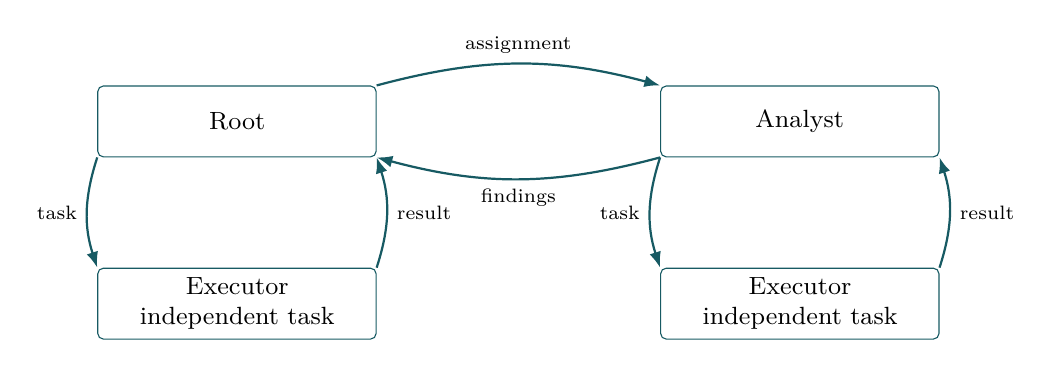
\begin{tikzpicture}[
  box/.style={draw=accent,rounded corners=2pt,align=center,font=\small,
    minimum height=9mm,text width=33mm},
  arrow/.style={-{Latex[length=2mm]},draw=accent,thick}]
\node[box] (root) {Root};
\node[box,right=36mm of root] (analyst) {Analyst};
\node[box,below=14mm of root] (rootexec) {Executor\\independent task};
\node[box,below=14mm of analyst] (analystexec) {Executor\\independent task};
\draw[arrow] (root.north east) to[bend left=15] node[above,font=\scriptsize]{assignment} (analyst.north west);
\draw[arrow] (analyst.south west) to[bend left=15] node[below,font=\scriptsize]{findings} (root.south east);
\draw[arrow] (root.south west) to[bend right=18] node[left,font=\scriptsize]{task} (rootexec.north west);
\draw[arrow] (rootexec.north east) to[bend right=18] node[right,font=\scriptsize]{result} (root.south east);
\draw[arrow] (analyst.south west) to[bend right=18] node[left,font=\scriptsize]{task} (analystexec.north west);
\draw[arrow] (analystexec.north east) to[bend right=18] node[right,font=\scriptsize]{result} (analyst.south east);
\end{tikzpicture}
\caption{Runtime delegation and return loops. Each executor assignment has its
own context and returns evidence to its requesting parent. This benchmark uses
the direct Root-to-executor route with local Root dispatch and low execution
effort.}
\label{fig:path}
\end{figure}

\section{Experimental protocol}

\subsection{Tasks and outcome definition}

SWE-bench evaluates issue resolution in real repositories through executable
tests~\cite{swebench}. We use every entry, in original order, from
\texttt{MariusHobbhahn/swe-bench-verified-mini}, a community-selected dataset
containing 50 tasks drawn from SWE-bench Verified~\cite{mini}. The fixed
manifest hash is published with the result summaries.

Each task starts from its specified base commit and issue text. Agent access
is restricted to the provided repository, issue and preinstalled dependencies.
The agent container has networking disabled. Host-side infrastructure relays
model requests, keeping model credentials outside the task container. Official
evaluation uses the generated prediction against the SWE-bench task tests.

Let $r_i=1$ for an official resolved result and $r_i=0$ otherwise. An unfinished
task also receives $r_i=0$. The reported score is
\begin{equation}
  R = \frac{1}{50}\sum_{i=1}^{50} r_i.
\end{equation}
HCCA has 49 official reports, with 36 resolved and 13 unresolved outcomes.
Its unfinished task, \texttt{sphinx-doc\_\_sphinx-8721}, receives zero credit.
All 17 requests and the consumed usage of that task remain in the HCCA totals.
Both DSH runs have official results for all 50 tasks.

\subsection{Configurations and provenance}

HCCA uses the frozen v7 runtime, with 41 runtime files and 10 original
operations files verified against its source manifest. Its run-local adapter
selects GXWTF and \texttt{deepseek-v4.1-flash}, with two concurrent task slots.
The HCCA role policy configures thinking/planning and analysts at high effort,
and execution/reading at low. The measured direct-execution path produces
1,301 low requests and zero high requests.

Both DSH runs use the same frozen SDK version 0.1.5-rc.1 and
\texttt{sdk-minimal} profile~\cite{dsh}. The historical high run uses GXWTF's
\texttt{deepseek-v4.1-flash} alias and two concurrent tasks. The new low run
uses the official \texttt{deepseek-flash} alias, displayed by the provider as
DeepSeek-V4.1-Flash, and four concurrent tasks. Inspection of all 100 DSH
sessions records the same initial system text, the same bash tool schema and
a 1,000,000-token model-context setting in both runs. Each session has one
system message, and the observed compaction-event count is zero. The two
aliases have distinct catalog metadata, with a fixed text prompt and tool
schema in these measured sessions.

\begin{table}[ht]
\centering
\small
\setlength{\tabcolsep}{3pt}
\begin{tabular}{p{44mm}p{37mm}p{37mm}p{37mm}}
\toprule
Setting & HCCA v7 (low) & DSH minimal low & DSH minimal high\\
\midrule
Provider & GXWTF & DeepSeek official & GXWTF\\
Model alias & \texttt{deepseek-v4.1-flash} & \texttt{deepseek-flash} & \texttt{deepseek-v4.1-flash}\\
Concurrent tasks & 2 & 4 & 2\\
Measured model effort & low & low & high\\
Initial model-planning stage & omitted & minimal loop & minimal loop\\
Context setting & 524,288 soft estimate & 1,000,000 model window & 1,000,000 model window\\
Run date, UTC & November 12 & November 13 & November 11\\
Generation budget per task & 4,800 seconds & 4,800 seconds & 4,800 seconds\\
Client output token ceiling & omitted & omitted & omitted\\
Temperature and seed & omitted & omitted & server defaults\\
\bottomrule
\end{tabular}
\caption{Recorded configurations in November 2026. Each task has at most one
outstanding model request. HCCA's local soft context estimate and DSH's model
window describe their respective context policies.}
\label{tab:config}
\end{table}

The HCCA executor starts directly, with unlimited executor rounds and shared
calls subject to the active-runner deadline. Preparation and official
evaluation occur outside generation budgets. The source records retain the
run-local GXWTF certificate-compatibility setting for the historical runs and
enabled certificate validation for the new official run.

\subsection{Accounting and the failed provider segment}

Resolution comes from explicit official report booleans. We reconcile the
new DSH run's host relay with its SDK request observer. All 1,061 physical
requests return HTTP 200 with complete base usage and cache splits. Request
body hashes and token totals agree between the two observers. HCCA's 1,301
requests also have complete usage. Historical DSH high has 2,014 requests,
including 2,013 complete usage records and one record with missing cache
splits. Its token aggregates below sum the complete records, yielding a
known-complete cost lower bound.

The current test first attempts \texttt{django\_\_django-11790} on GXWTF.
All six physical requests return HTTP 500 with unknown usage. The subsequent
official full-manifest run starts all 50 tasks independently. The current
testing expenditure comprises 1,061 official requests plus these six failed
GXWTF requests, for 1,067 in total. Its exact token totals and normalized cost
remain unknown, with known-complete cost at least \$\LCost{}. The completed
official 50-task segment has its own exact normalized cost of \$\LCost{}.

We apply common off-peak rates in USD per million tokens of 0.003 for cached
input, 0.15 for uncached input and 0.60 for output~\cite{prices}. For counts
$I_c$, $I_u$ and $O$, normalized cost is
\begin{equation}
  C = \frac{0.003 I_c + 0.15 I_u + 0.60 O}{10^6}.
\label{eq:cost}
\end{equation}
Provider-reported reasoning tokens are included in $O$ once. Actual provider
billing remains unknown and has its own field in the public summaries.

\section{Results}

\begin{table}[ht]
\centering
\small
\setlength{\tabcolsep}{4pt}
\begin{tabular}{lrrr}
\toprule
Metric & HCCA v7 (low) & DSH minimal low & DSH minimal high\\
\midrule
Resolved / all tasks & 36 / 50 & 34 / 50 & 35 / 50\\
Officially evaluated & 49 & 50 & 50\\
Unfinished & 1 & 0 & 0\\
Actual model requests & \HRequests{} & \LRequests{} & \BRequests{}\\
Complete / incomplete usage & 1,301 / 0 & 1,061 / 0 & 2,013 / 1\\
Input tokens & \HInput{} & \LInput{} & $\geq$\BInput{}\\
Cached input tokens & \HCached{} & \LCached{} & $\geq$\BCached{}\\
Uncached input tokens & \HMiss{} & \LMiss{} & $\geq$\BMiss{}\\
Cached share of complete input & \HCachePct{}\% & \LCachePct{}\% & \BCachePct{}\%\\
Output tokens, including reasoning & \HOutput{} & \LOutput{} & $\geq$\BOutput{}\\
Reasoning in complete records & \HReasoning{} & \LReasoning{} & \BReasoning{}\\
Other output in complete records & \HOtherOutput{} & \LOtherOutput{} & \BOtherOutput{}\\
Normalized cost, USD & \HCost{} & \LCost{} & $\geq$\BCost{}\\
\bottomrule
\end{tabular}
\caption{Fixed-manifest outcomes and usage. DSH low covers its completed official
50-task segment. The six failed GXWTF requests remain in the whole-attempt
accounting described in Section~3.3. DSH high token aggregates use its 2,013
complete records. All HCCA usage, including the unfinished task, is included.}
\label{tab:results}
\end{table}

\subsection{HCCA and DSH at low effort}

HCCA resolves 72\% of the manifest and DSH low resolves 68\%. Both resolve 33
tasks, HCCA alone resolves three, DSH low alone resolves one, and neither
resolves 13. HCCA's three additional successes are
\texttt{django\_\_django-11848}, \texttt{django\_\_django-11885} and
\texttt{django\_\_django-12308}. DSH low resolves
\texttt{sphinx-doc\_\_sphinx-8721}, the unfinished HCCA task.

For these complete 50-task accounting scopes, HCCA's normalized cost is
16.3\% higher than DSH low's. It consumes 25.8\% more input and 26.8\% more
output tokens, with 22.6\% more requests. Normalized cost per resolved task is
\$\HCostPerResolved{} for HCCA and \$\LCostPerResolved{} for DSH low.
These observations give two additional resolved tasks at higher recorded cost
for the HCCA configuration.

\subsection{Historical high-effort reference}

DSH high resolves 35 tasks and DSH low resolves 34. Both resolve 33 tasks,
high alone resolves two, low alone resolves one, and neither resolves 14.
The low run's normalized cost is at most 18.09\% of the high run's
known-complete cost, a reduction of at least 81.9\%. Its output is 87.3\%
lower than the high run's complete-record output, and its recorded reasoning
is 90.1\% lower. The historical HCCA--DSH high comparison retains its original
36 versus 35 outcomes and corresponding cost records~\cite{historical}.

\begin{figure}[ht]
\centering
\begin{minipage}[t]{.32\linewidth}\centering
\textbf{\scriptsize Input tokens (millions)}\\[2pt]
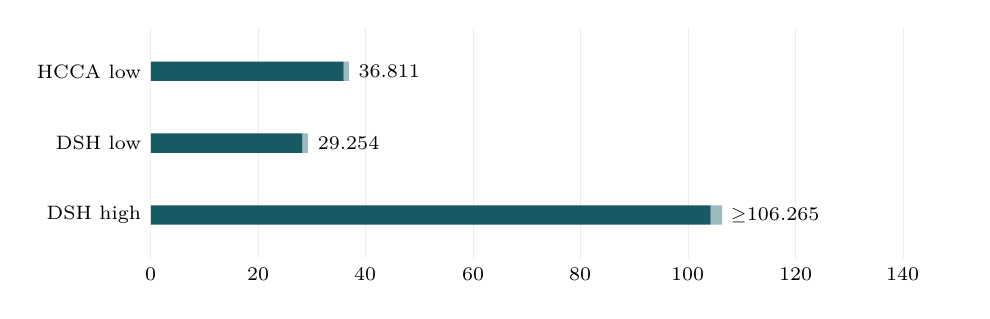
\begin{tikzpicture}\begin{axis}[
width=.98\linewidth,height=45mm,xbar stacked,bar width=7pt,
symbolic y coords={DSH high,DSH low,HCCA low},ytick=data,
ymin={[normalized]-0.6},ymax={[normalized]2.6},xmin=0,xmax=150.9,
axis lines*=left,axis line style={draw=none},tick style={draw=none},
tick label style={font=\scriptsize},xmajorgrids,grid style={gray!15},enlarge y limits=false]
\addplot[fill=accent,draw=none] coordinates {(35.849984,{HCCA low}) (28.189696,{DSH low}) (104.137856,{DSH high})};
\addplot[fill=cachelight,draw=none] coordinates {(0.960532,{HCCA low}) (1.063901,{DSH low}) (2.127590,{DSH high})};
\node[anchor=west,font=\scriptsize] at (axis cs:36.810516,HCCA low){36.811};
\node[anchor=west,font=\scriptsize] at (axis cs:29.253597,DSH low){29.254};
\node[anchor=west,font=\scriptsize] at (axis cs:106.265446,DSH high){$\geq$106.265};
\end{axis}\end{tikzpicture}
{\scriptsize \textcolor{accent}{Cached}\quad \textcolor{cachelight}{Uncached}}
\end{minipage}
\hfill
\begin{minipage}[t]{.32\linewidth}\centering
\textbf{\scriptsize Output tokens (millions)}\\[2pt]
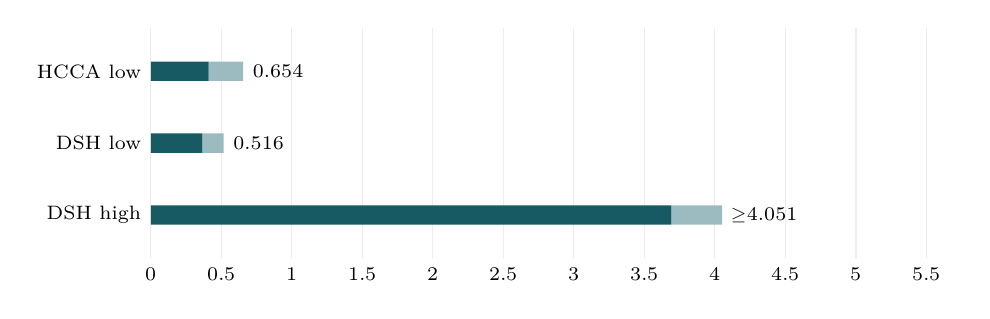
\begin{tikzpicture}\begin{axis}[
width=.98\linewidth,height=45mm,xbar stacked,bar width=7pt,
symbolic y coords={DSH high,DSH low,HCCA low},ytick=data,
ymin={[normalized]-0.6},ymax={[normalized]2.6},xmin=0,xmax=5.7522,
axis lines*=left,axis line style={draw=none},tick style={draw=none},
tick label style={font=\scriptsize},xmajorgrids,grid style={gray!15},enlarge y limits=false]
\addplot[fill=accent,draw=none] coordinates {(0.408903,{HCCA low}) (0.365085,{DSH low}) (3.690753,{DSH high})};
\addplot[fill=cachelight,draw=none] coordinates {(0.245401,{HCCA low}) (0.151064,{DSH low}) (0.360084,{DSH high})};
\node[anchor=west,font=\scriptsize] at (axis cs:0.654304,HCCA low){0.654};
\node[anchor=west,font=\scriptsize] at (axis cs:0.516149,DSH low){0.516};
\node[anchor=west,font=\scriptsize] at (axis cs:4.050837,DSH high){$\geq$4.051};
\end{axis}\end{tikzpicture}
{\scriptsize \textcolor{accent}{Reasoning}\quad \textcolor{cachelight}{Other output}}
\end{minipage}
\hfill
\begin{minipage}[t]{.32\linewidth}\centering
\textbf{\scriptsize Normalized cost (USD)}\\[2pt]
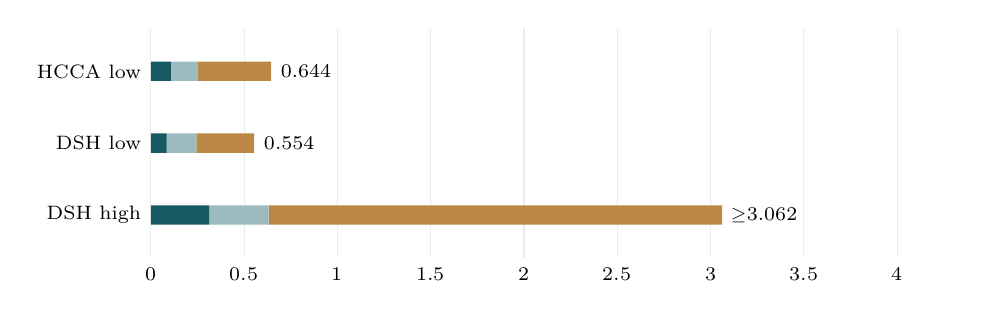
\begin{tikzpicture}\begin{axis}[
width=.98\linewidth,height=45mm,xbar stacked,bar width=7pt,
symbolic y coords={DSH high,DSH low,HCCA low},ytick=data,
ymin={[normalized]-0.6},ymax={[normalized]2.6},xmin=0,xmax=4.3482,
axis lines*=left,axis line style={draw=none},tick style={draw=none},
tick label style={font=\scriptsize},xmajorgrids,grid style={gray!15},enlarge y limits=false]
\addplot[fill=accent,draw=none] coordinates {(0.107549952,{HCCA low}) (0.084569088,{DSH low}) (0.312413568,{DSH high})};
\addplot[fill=cachelight,draw=none] coordinates {(0.144079800,{HCCA low}) (0.159585150,{DSH low}) (0.319138500,{DSH high})};
\addplot[fill=outputgold,draw=none] coordinates {(0.392582400,{HCCA low}) (0.309689400,{DSH low}) (2.430502200,{DSH high})};
\node[anchor=west,font=\scriptsize] at (axis cs:0.644212152,HCCA low){0.644};
\node[anchor=west,font=\scriptsize] at (axis cs:0.553843638,DSH low){0.554};
\node[anchor=west,font=\scriptsize] at (axis cs:3.062054268,DSH high){$\geq$3.062};
\end{axis}\end{tikzpicture}
{\scriptsize \textcolor{accent}{Cached input}\quad \textcolor{cachelight}{Uncached input}\quad \textcolor{outputgold}{Output}}
\end{minipage}

\caption{Input, output and normalized-cost composition for the three measured
configurations. DSH low shows the official 50-task segment. DSH high shows
known-complete lower bounds. Reasoning is already included in output.}
\label{fig:usage}
\end{figure}

The official low run's model-request window is 01:36:48.459769 to
02:10:11.148351 UTC on November 13, 2026. The final complete state is recorded
at 02:11:31.541700 UTC. Historical HCCA's generation-and-evaluation phase ends
at 12:58:53 UTC on November 12, approximately 60 minutes after launch. The
DSH high model-request window is 04:13:28 to 09:00:27 UTC on November 11.
These timings retain their different scopes, provider conditions and task
concurrency.

\section{Interpreting token consumption}

\subsection{Request count, input size and cache reuse}

Total input sums prompt sizes across requests. HCCA averages approximately
28,294 input tokens per request, DSH low 27,572, and DSH high 52,790 across
its complete records. The HCCA--DSH low input gap combines more requests with
a slightly larger average request. Shared role prefixes and independent worker
histories describe HCCA's implementation, while the observed aggregates give
the configuration's measured consumption.

The cached shares of complete input are \HCachePct{}\% for HCCA,
\LCachePct{}\% for DSH low and \BCachePct{}\% for DSH high. HCCA consumes
960,532 uncached input tokens, compared with 1,063,901 for DSH low, alongside
higher total input. At the common rates, HCCA's cached-input, uncached-input
and output components cost approximately \$0.107550, \$0.144080 and
\$0.392582. DSH low's corresponding components are \$0.084569, \$0.159585
and \$0.309689. Output accounts for approximately 91.7\% of the additional
normalized cost of HCCA over DSH low.

Provider cache counters establish aggregate reuse under each run's serving
conditions. Their causal relationship to shared instructions and worker
isolation requires direct prefix-level measurements under matched conditions.

\subsection{Reasoning and other output}

HCCA's \HOutput{} output tokens include \HReasoning{} reasoning tokens and
\HOtherOutput{} other output tokens. DSH low records \LOutput{} output,
including \LReasoning{} reasoning and \LOtherOutput{} other output. The gap
comprises 43,818 reasoning tokens and 94,337 other output tokens, contributing
31.7\% and 68.3\% of the total output difference. Other output is derived by
subtraction and can include visible text and tool-call arguments.

The two low-effort configurations therefore differ in both reasoning volume
and other generated material. Their tools, prompts and repair trajectories
also differ. In the historical comparison with DSH high, reasoning accounts
for approximately 96.6\% of the recorded output difference. The new low run
changes the empirical output comparison and its interpretation.

\section{Limitations and reproducibility}

The observations come from one run per configuration on a fixed 50-task
community-selected subset. Earlier HCCA versions were developed and evaluated
on the same manifest. The two-task HCCA advantage over DSH low and one-task
DSH high advantage over low carry the variability of these single runs.
Matched repetitions on independently specified tasks would measure that
variability.

The two low configurations share recorded effort, with different providers,
model aliases, task concurrency, prompts, tools and execution policies. The
two DSH runs share their SDK, minimal profile, effective context setting,
system text and bash schema, while effort, provider, alias, concurrency and
run date vary. These factors bound attribution of resolution and token changes
to any individual mechanism.

The HCCA measurement exercises direct execution with local Root dispatch.
Reader isolation, multi-level decomposition, multiple collaborating workers
and interactive user guidance have their own evaluation scope. The current
Official distribution also includes packaging and Windows/DSH integration
work beyond the measured frozen snapshot.

Public records include the fixed manifest identity, source hashes, per-task
outcomes, request counts, complete token accounting and both provider
segments of the new test~\cite{artifacts}. The independent audit reconciles all
1,061 official requests and verifies the frozen 13-file operations manifest.
The missing usage of six GXWTF failures and one historical high record remains
explicitly unknown. Versioned November 12 artifacts preserve the earlier
comparison~\cite{historical}. Re-execution requires the dataset, prepared
repository images, provider access and the matching runtime snapshot.

\newpage
\section{Conclusion}

On the fixed Verified Mini 50-task manifest, frozen HCCA v7 at low effort
resolves 36 tasks at \$\HCost{} normalized cost, and the new official DSH
minimal low run resolves 34 at \$\LCost{}. HCCA consumes more input and
output, with 16.3\% higher normalized cost for two additional resolved tasks.
The historical DSH minimal high run resolves 35 at a known-complete cost of
at least \$\BCost{}. DSH low's official 50-task segment costs at least 81.9\%
less than that historical high reference. All three configurations achieve
substantial input-cache reuse. The new test's six failed GXWTF requests keep
its entire expenditure unknown. The completed official segment supplies a
fully accounted low-effort reference for subsequent configuration studies.

\begin{thebibliography}{9}
\small
\raggedright
\bibitem{swebench}
Carlos E. Jimenez, John Yang, Alexander Wettig, Shunyu Yao, Kexin Pei,
Ofir Press and Karthik R. Narasimhan.
\emph{SWE-bench\textup{:} Can Language Models Resolve Real-World GitHub Issues?}
ICLR, 2024. \url{https://openreview.net/forum?id=VTF8yNQM66}.

\bibitem{mini}
Marius Hobbhahn. \emph{swe-bench-verified-mini}. Dataset repository.
\url{https://huggingface.co/datasets/MariusHobbhahn/swe-bench-verified-mini}.
Fixed task manifest and data hashes accompany this report.

\bibitem{dsh}
DeepSeek-AI. \emph{DeepSeek Harness}. 2026.
\url{https://github.com/deepseek-ai/deepseek-harness}.
The experiment uses SDK 0.1.5-rc.1 with the minimal profile.

\bibitem{prices}
DeepSeek. \emph{Models and Pricing}.
\url{https://api-docs.deepseek.com/quick_start/pricing/}.
Common off-peak rates are frozen in the published accounting.

\bibitem{historical}
HCCA Project. \emph{Frozen-v7 Verified Mini results and accounting}.
November 12, 2026.
\url{https://github.com/klarisaka/HCCA-Official/blob/main/reports/verified50-hcca-v7-vs-dsh-2026-11-12-summary.json}.

\bibitem{artifacts}
HCCA Project. \emph{DSH minimal low Verified Mini results and accounting}.
November 13, 2026.
\url{https://github.com/klarisaka/HCCA-Official/blob/main/reports/verified50-dsh-minimal-low-2026-11-13-summary.json}.
Runtime distribution at \url{https://github.com/klarisaka/HCCA-Official}.
\end{thebibliography}

\end{document}
